\begin{frame}{E1 - Comparison to Seq. Baseline: \small{$\Sigma(\mathsf{GDB_A}, s(120, 0.02), f, c)$}}
\begin{figure}
    \centering
    \hspace{-1.7cm}
    \begin{subfigure}{0.45\textwidth}
        \centering
        \stackinset{c}{}{t}{0.4cm}{
            \shortstack{\texttt{MRT} (s) \\ Mean Response Time}
        }{
        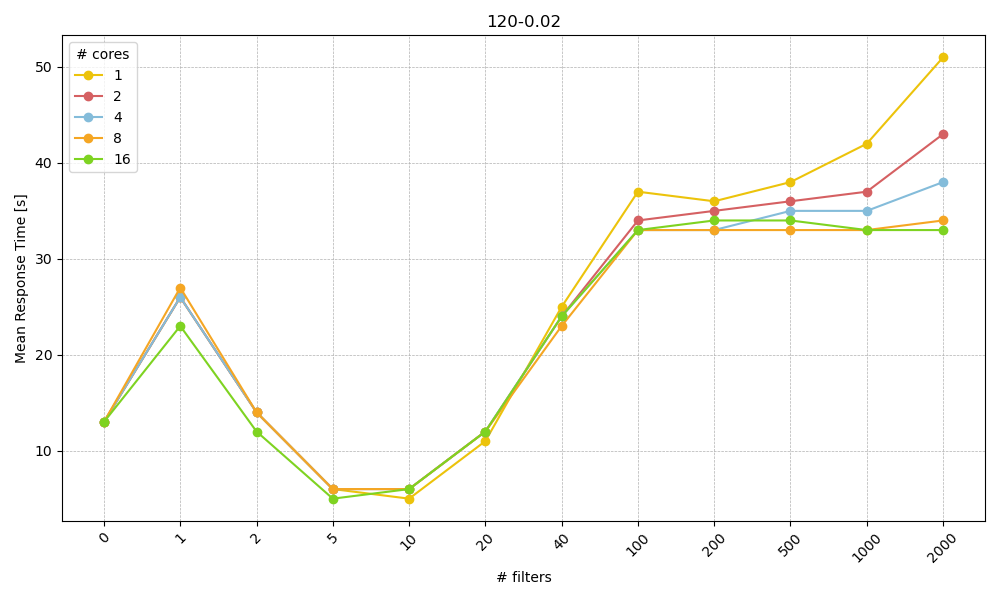
\includegraphics[scale=0.25]{images/4-Experiments/NRT/small/120-0.02/combined/mrt-1.png}
        }
    \end{subfigure}
    \hspace{1.2cm}
    \begin{subfigure}{0.45\textwidth}
        \centering
        \stackinset{c}{}{t}{0.4cm}{
            \shortstack{\texttt{ET} (s) \\ Execution Time}
        }{
        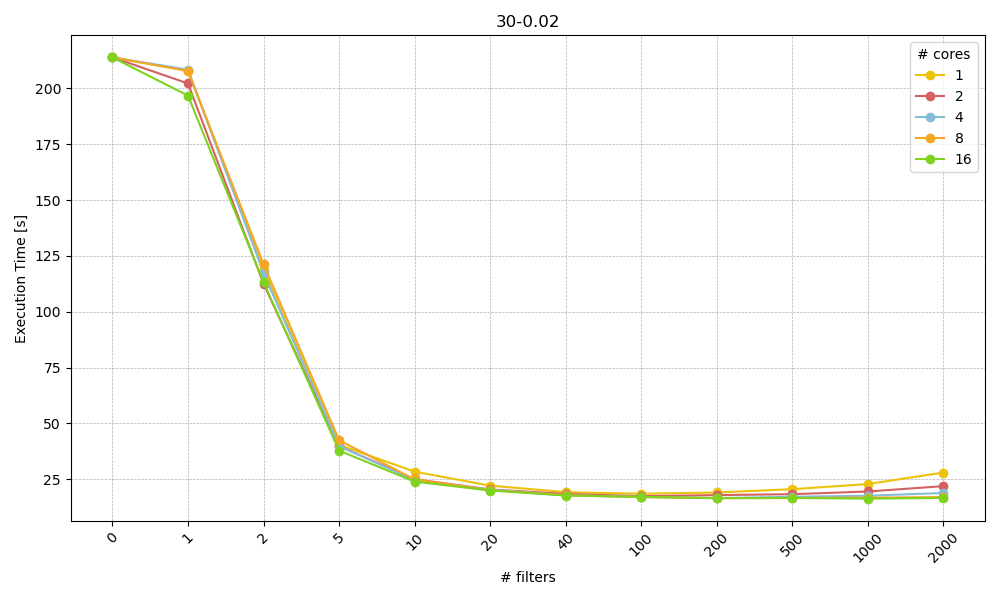
\includegraphics[scale=0.25]{images/4-Experiments/NRT/small/120-0.02/combined/execTime-1.png}
        }
        %\caption{\texttt{ET} (s)}
    \end{subfigure}
    \vspace{0.1cm}
    \hspace{-1.7cm}
    \begin{subfigure}{0.45\textwidth}
        \centering
        \stackinset{c}{}{t}{2.3cm}{
            \shortstack{\texttt{dief@t} \\ \emph{diefficiency}}
        }{
        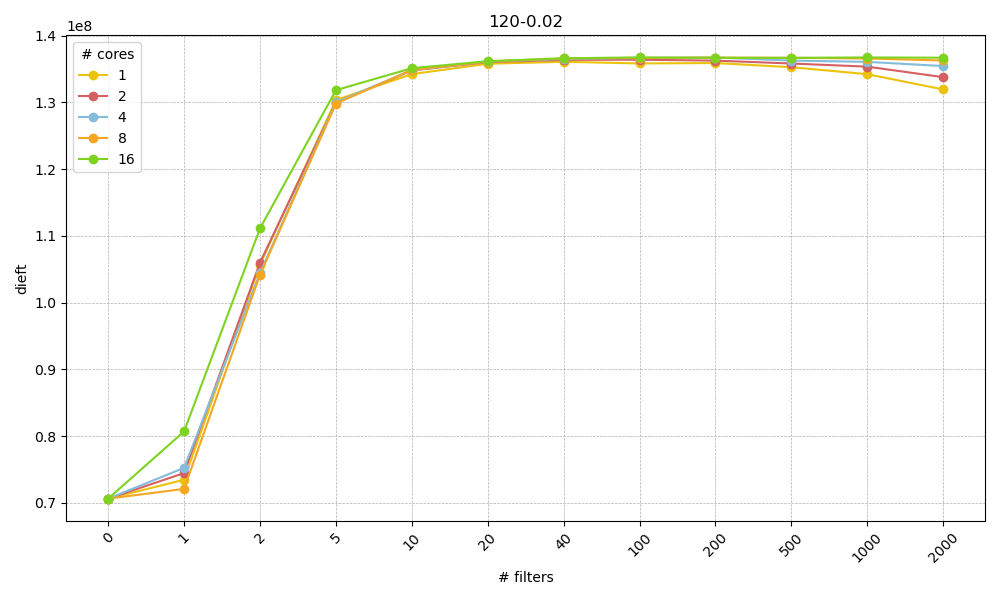
\includegraphics[scale=0.25]{images/4-Experiments/NRT/small/120-0.02/combined/dieft-1.png}
        }
        %\caption{\texttt{dief@t}}
    \end{subfigure}
    \hspace{1.2cm}
    \begin{subfigure}{0.45\textwidth}
        \centering
        \stackinset{c}{}{t}{2.3cm}{
            \shortstack{\texttt{T} (checks/s) \\ Throughput}
        }{
        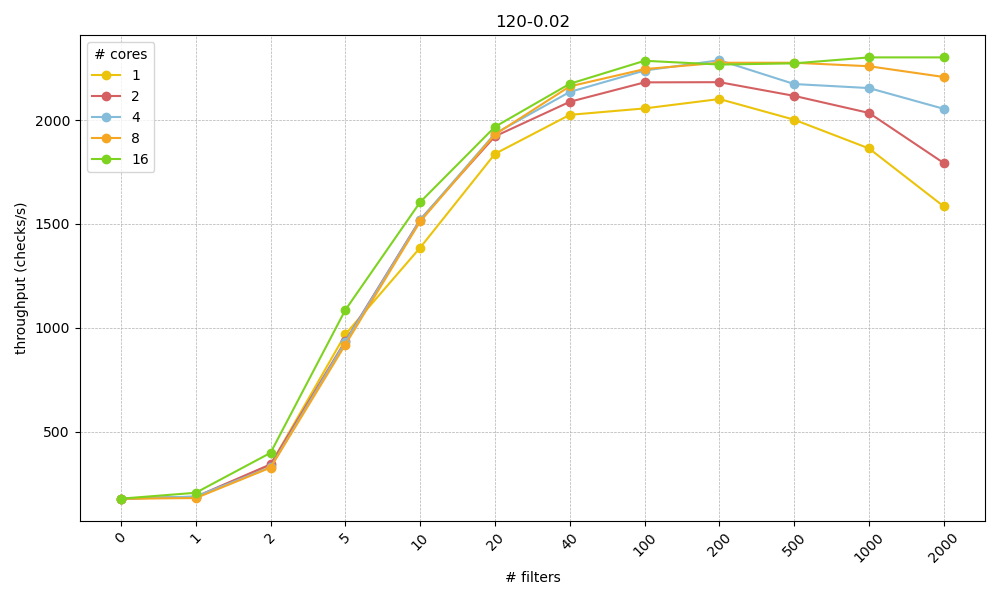
\includegraphics[scale=0.25]{images/4-Experiments/NRT/small/120-0.02/combined/throughput-1.png}
        }
        %\caption{\texttt{T} (checks/s)}
    \end{subfigure}
\end{figure}
\end{frame}

\begin{frame}{E1 - Num. Filters Configuration: \small{$\Sigma(\mathsf{GDB_B}, s(15, 0.03), f, 8)$}}
\begin{columns} % Create two columns
    % Left column for the item list
    \begin{column}{0.45\textwidth}
    \begin{itemize}
        \item Best $\texttt{MRT}$ for $f=5$-$10$.
        \vspace{1em}
        \item Best \texttt{ET}, \texttt{dief@t} for higher $f$'s.
    \end{itemize}
    \end{column}

    % Right column for the image
    \begin{column}{0.7\textwidth}
        \centering
    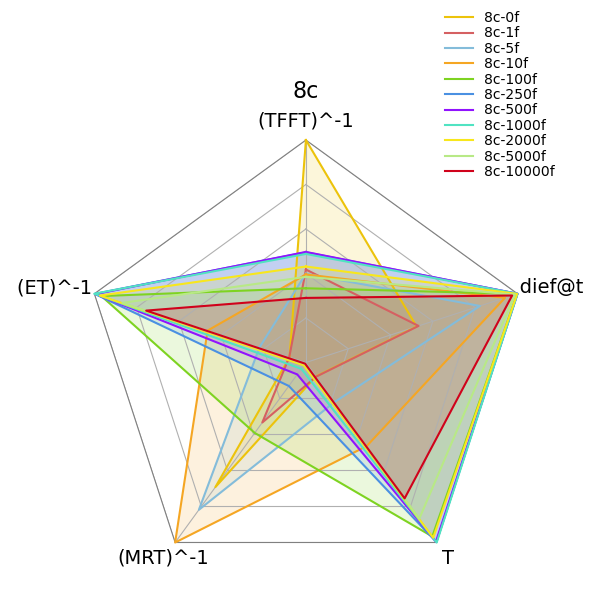
\includegraphics[scale=0.5]{images/4-Experiments/NRT/medium/15-0.03/fixedcores/8c/radar-dieft.png}
    \end{column}
\end{columns}

\end{frame}


\begin{frame}{E1 - Num. Filters Configuration: \small{$\Sigma(\mathsf{GDB_B}, s(15, 0.03), f, 8)$}}
\begin{itemize}
    \item Check results trace for $\Sigma(\mathsf{GDB_B}, s(15, 0.03), f, 8)$.
    \item \textbf{Higher} number of \textbf{filters} outperform in \textbf{continuous behavior}.
\end{itemize}
\vspace{-1cm}
\begin{figure}
    \hspace{-0.70cm}
    \centering
    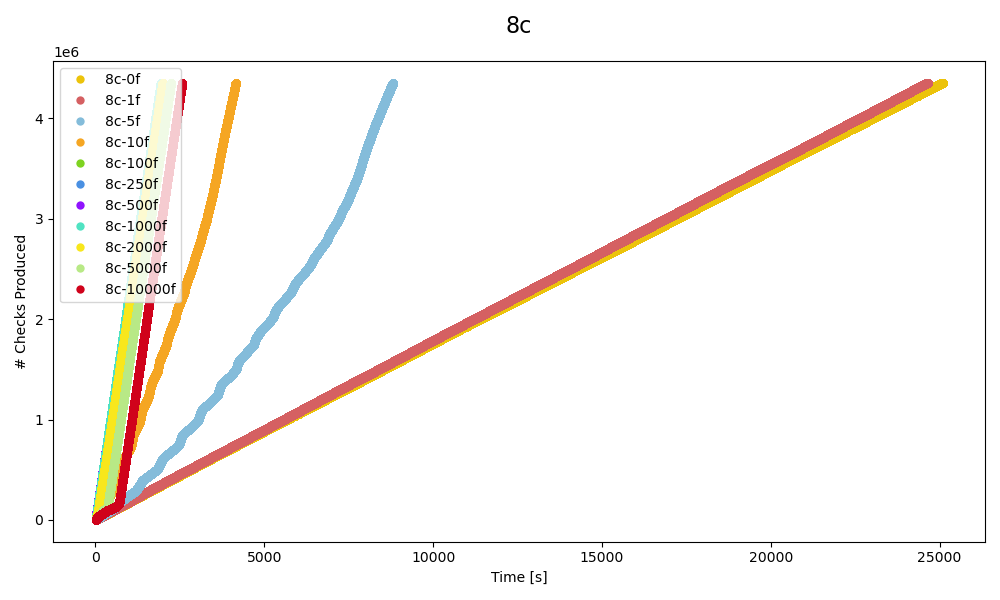
\includegraphics[scale=0.45]{images/4-Experiments/NRT/medium/15-0.03/fixedcores/8c/traces.png}
    \label{img:exps-medium-15D-8c-trace}
\end{figure}
\end{frame}


\begin{frame}{E1 - Num. Filters Configuration: \small{$\Sigma(\mathsf{GDB_B}, s(7, 0.03), f, c)$}}
\begin{itemize}
    \item \textbf{Degradation} of the behavior of the configurations with \textbf{high number of filters} $f$ for \textbf{low} number of \textbf{cores} $c$ executions.
    \item Possible causes: (i) \texttt{goroutines} overhead; (ii) Neo4j multiple parallel connections overhead; (iii) Sink ($\mathsf{Sk}$) stage bottleneck.
\end{itemize}
\begin{figure}
    \centering
    \hspace*{-1.6cm} % Move content to the left
    \begin{subfigure}{0.5\textwidth}
        \centering
        \includegraphics[scale=0.44]{images/4-Experiments/NRT/medium/7-0.03/fixedcores/1c/execTime.png}
    \end{subfigure}
    \hspace*{1cm} 
    \begin{subfigure}{0.5\textwidth}
        \centering
        \includegraphics[scale=0.44]{images/4-Experiments/NRT/medium/7-0.03/fixedcores/8c/execTime.png}
    \end{subfigure}
\end{figure}
\end{frame}

\begin{frame}{E1 - Achieved Performance (\texttt{RT} and \texttt{MRT})}

\begin{itemize}
    \item Achieved \textbf{low} and \textbf{constant} \texttt{RT} (Response Time) values.
    \item For the \textbf{largest tested streams} for each $g$ the \texttt{MRT} achieved is around
    5-6 s for $\Sigma(\mathsf{GDB_A}, s(120, 0.02), f, c)$ and around 10s for $\Sigma(\mathsf{GDB_B}, s(15, 0.03), f, c)$.
\end{itemize}
\vspace{1em}
\begin{minipage}{0.48\textwidth}
\scalebox{0.7}{ 
    \begin{tabular}{|c||c|c|c|c|c|}
        \hline
        \multicolumn{6}{|c|}{\textbf{MRT (s) for} $\Sigma(\mathsf{GDB_A}, s(120, 0.02), f, c)$} \\
        \hline
        \multicolumn{6}{|c|}{Number of Cores} \\
        \hline
        \textbf{\# Filters} & \textbf{1} & \textbf{2} & \textbf{4} & \textbf{8} & \textbf{16} \\
        \hline
        $\mathsf{0}$     & 13  & 13  & 13  & 13  & 13  \\
         $\mathsf{1}$     & 26  & 26  & 26  & 27  & 23  \\
         $\mathsf{2}$     & 14  & 14  & 14  & 14  & 12  \\
         \rowcolor{green}$\mathsf{5}$     & 6   & 6   & 6   & 6   & 5   \\
         \rowcolor{green}$\mathsf{10}$    & 5   & 6   & 6   & 6   & 6   \\
         $\mathsf{20}$    & 11  & 12  & 12  & 12  & 12  \\
        $\mathsf{40}$   & 25  & 24  & 24  & 23  & 24  \\
         $\mathsf{100}$   & 37  & 34  & 33  & 33  & 33  \\
         $\mathsf{200}$   & 36  & 35  & 33  & 33  & 34  \\
        $\mathsf{500}$   & 38  & 36  & 35  & 33  & 34  \\
         $\mathsf{1000}$  & 42  & 37  & 35  & 33  & 33  \\
         $\mathsf{2000}$  & 51  & 43  & 38  & 34  & 33  \\
        \hline
    \end{tabular}
}
\end{minipage}
\hspace{0.1cm}
\begin{minipage}{0.48\textwidth}
\scalebox{0.7}{ 
    \begin{tabular}{|c||c|c|c|c|c|}
        \hline
        \multicolumn{6}{|c|}{\textbf{MRT (s) for $\Sigma(\mathsf{GDB_B}, s(15, 0.03), f, c)$}} \\
        \hline
        \multicolumn{6}{|c|}{Number of Cores} \\
        \hline
        \textbf{\# Filters} & \textbf{1} & \textbf{2} & \textbf{4} & \textbf{8} & \textbf{16} \\
        \hline
         $\mathsf{0}$     & 13   & 13   & 13   & 13   & 13   \\
         \rowcolor{green}$\mathsf{5}$     & 11   & 10   & 11   & 11   & 9    \\
         \rowcolor{green}$\mathsf{10}$    & 11   & 9    & 10   & 9   & 7    \\
         $\mathsf{100}$   & 33   & 40   & 29   & 23   & 37   \\
         $\mathsf{250}$   & 124  & 80   & 91   & 69   & 90   \\
         $\mathsf{500}$   & 221  & 161  & 134  & 136  & 138  \\
         $\mathsf{1000}$  & 502  & 301  & 267  & 256  & 263  \\
         $\mathsf{2000}$  & 937  & 702  & 618  & 562  & 554  \\
         $\mathsf{5000}$  & 2830 & 1732 & 1422 & 1124 & 1060 \\
         $\mathsf{10000}$ & 4957 & 2535 & 2025 & 1410 & 1249 \\
        \hline
    \end{tabular}
}
\end{minipage}
\end{frame}

\begin{frame}{E1 - Achieved Performance (\texttt{RT} and \texttt{MRT})}

\begin{itemize}
    \item Achieved \textbf{low} and \textbf{constant} \texttt{RT} (Response Time) values.
    \item E.g. Check results trace for $\Sigma(\mathsf{GDB_A}, s(120, 0.02), f, 16)$.
\end{itemize}
\begin{figure}
    \centering
    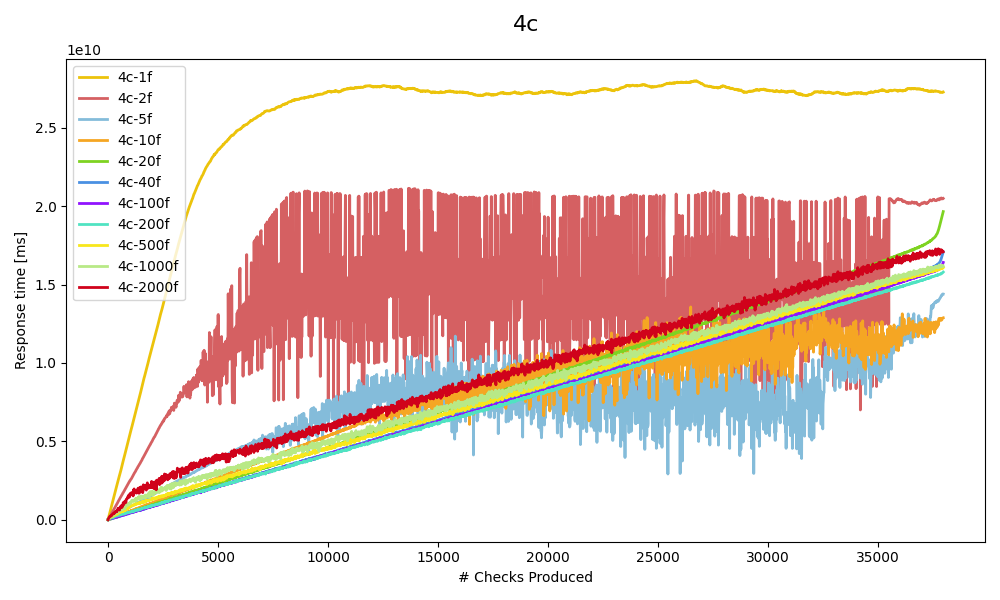
\includegraphics[scale=0.4]{images/4-Experiments/NRT/small/120-0.02/fixedcores/16c/traces-response-time-reduced.png}
\end{figure}
\end{frame}

\begin{frame}{E1 - Achieved Performance (\texttt{transactions/s})}

\begin{itemize}
    \item Achieved \textbf{large} transaction \textbf{processing rates}:
    \vspace{0.2em}
    \begin{itemize}
        \item $\Sigma(\mathsf{GDB_A}, s(120, 0.02), f, c)$: 2,500 transactions/s. 216,000,000 per day \textcolor{red}${\approx$ 200M}.
        \item $\Sigma(\mathsf{GDB_B}, s(15, 0.03), f, 16)$: 1,250 transactions/s. 108,000,000 per day. \textcolor{red}{$\approx$ 100M}.
    \end{itemize}
\end{itemize}
\begin{figure}
    \centering
    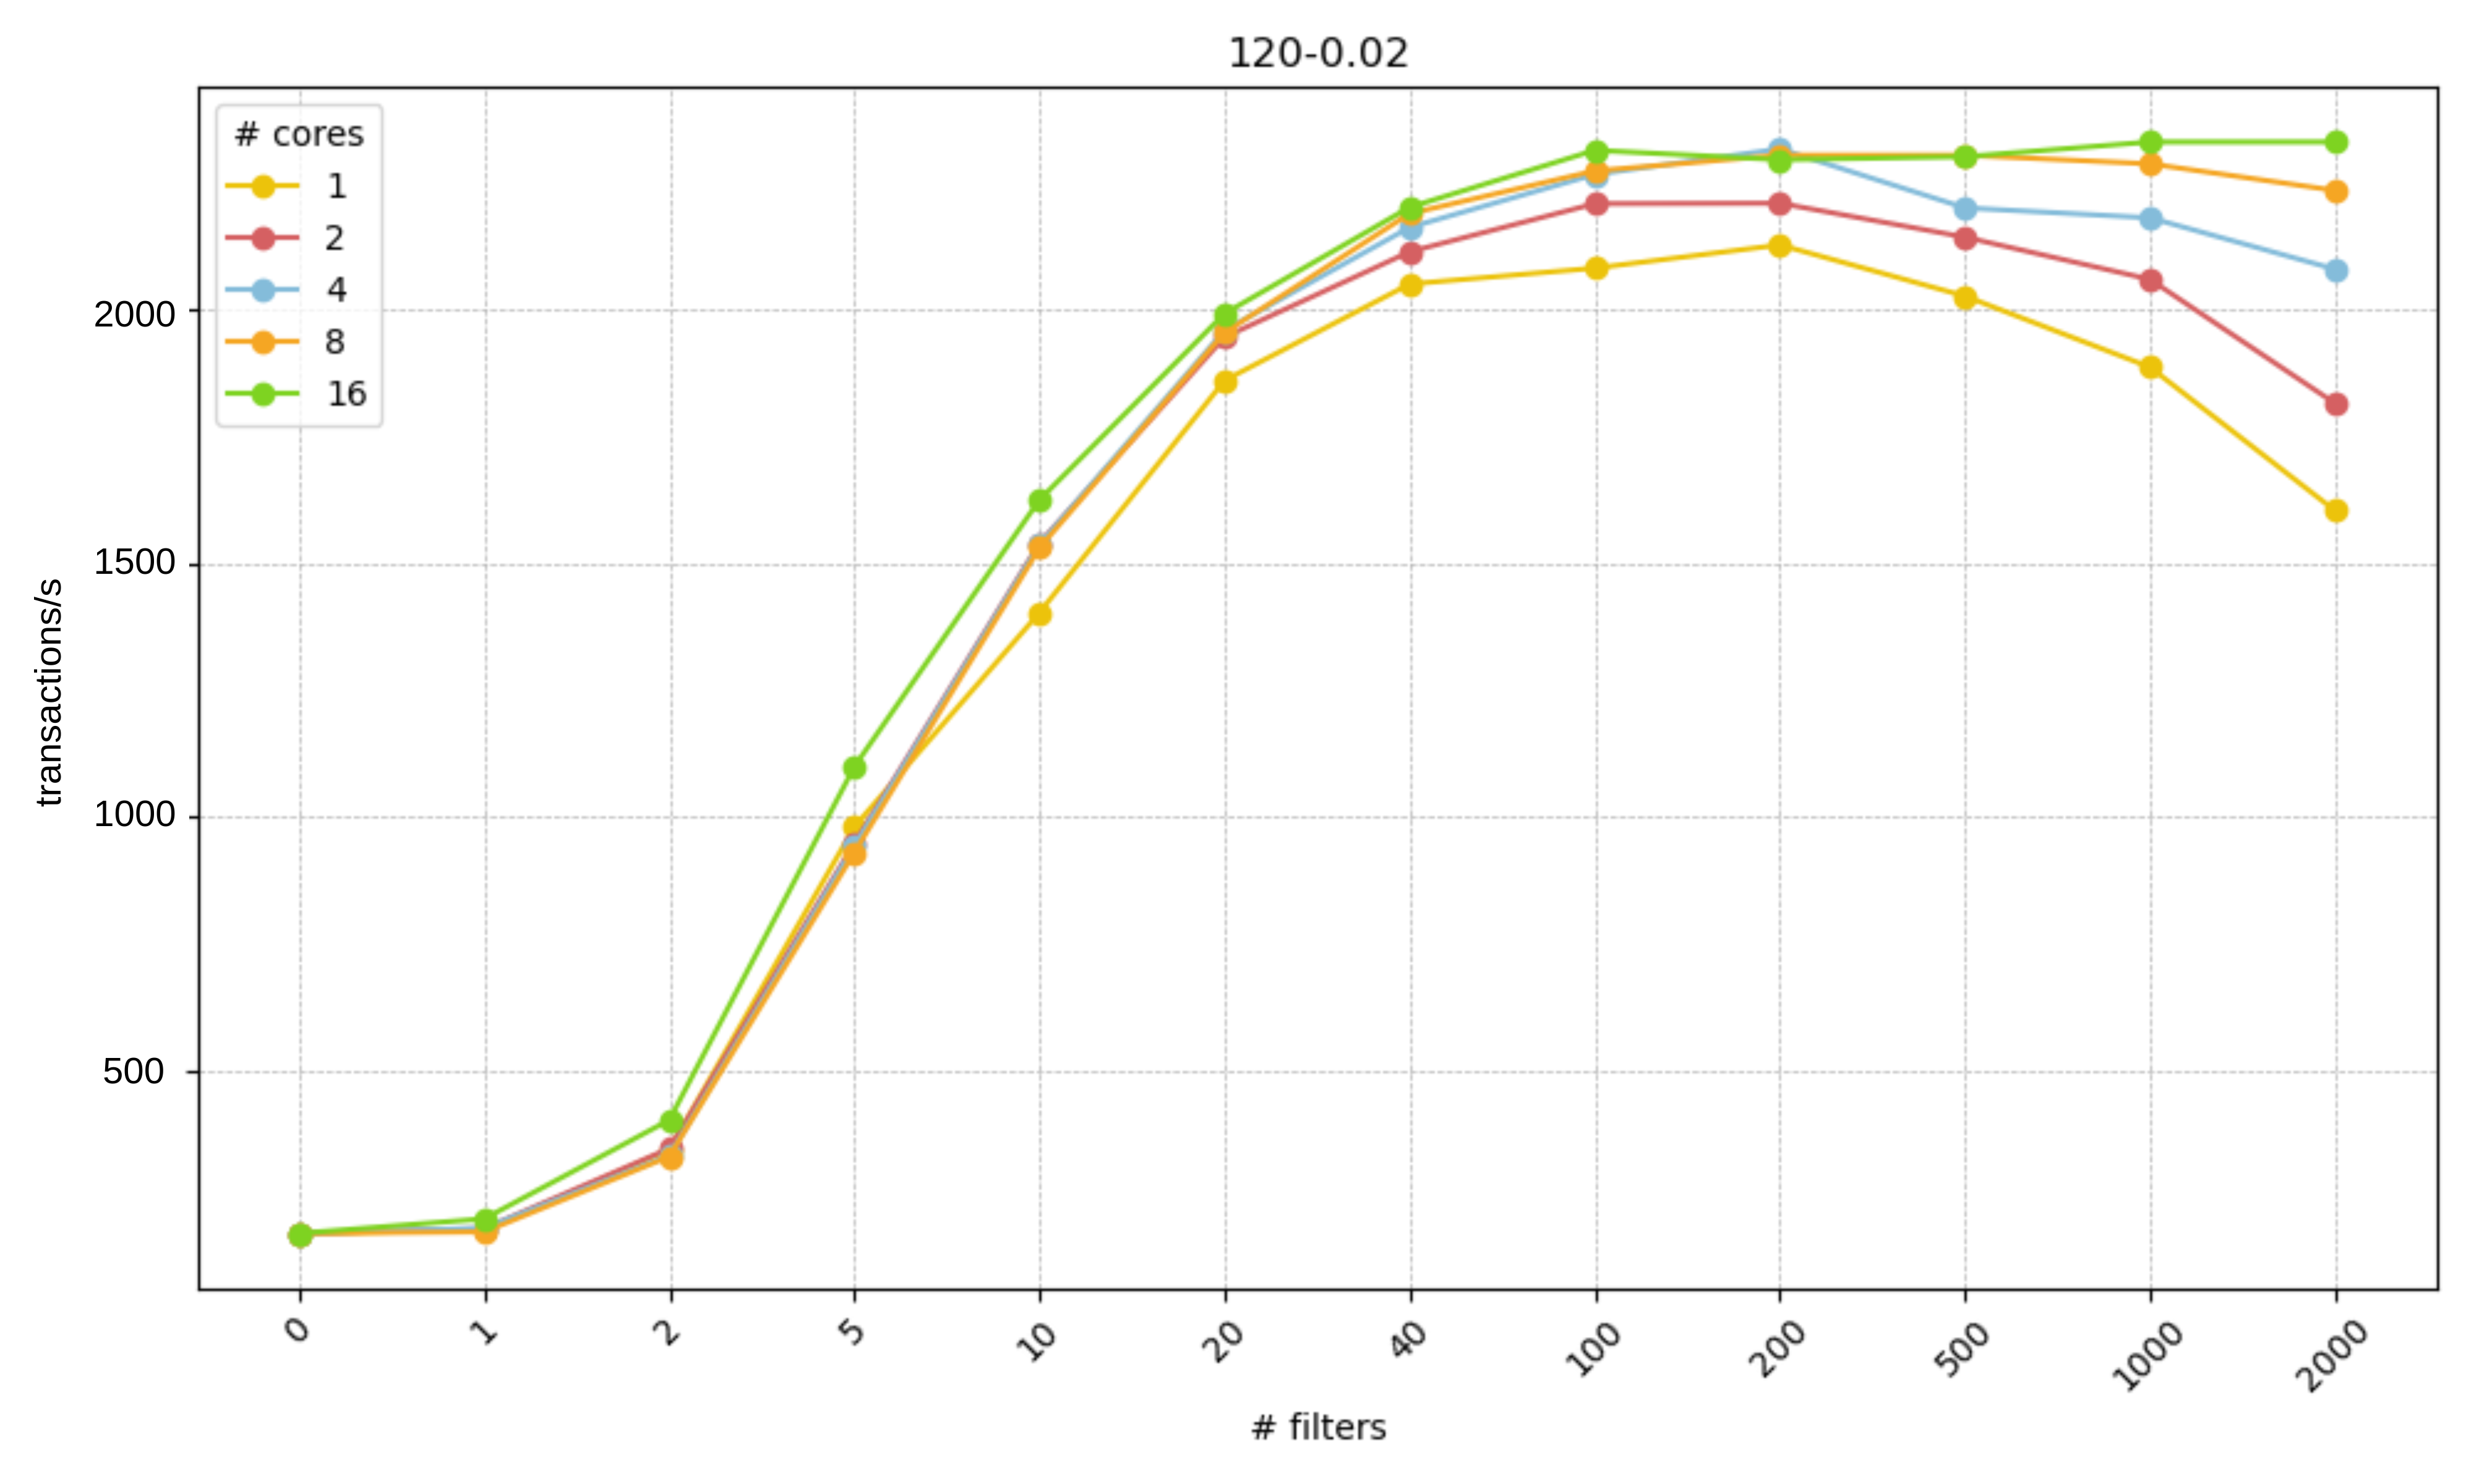
\includegraphics[scale=0.4]{figures/txpersec.png}
\end{figure}
\end{frame}

